\documentclass[twoside]{article}
\usepackage{aistats2014}
\usepackage{amsthm,amsmath}
\usepackage{amssymb}
\usepackage[boxed]{algorithm2e}
\usepackage{bm}
\usepackage{bbm}
\usepackage{url}
\usepackage{comment}
\usepackage{url}
\usepackage{multirow}
\usepackage{graphicx}
\usepackage{color}
\usepackage{tikz}

% If your paper is accepted, change the options for the package
% aistats2014 as follows:
%
%\usepackage[accepted]{aistats2014}
%
% This option will print headings for the title of your paper and
% headings for the authors names, plus a copyright note at the end of
% the first column of the first page.


\begin{document}

% If your paper is accepted and the title of your paper is very long,
% the style will print as headings an error message. Use the following
% command to supply a shorter title of your paper so that it can be
% used as headings.
%
%\runningtitle{I use this title instead because the last one was very long}

% If your paper is accepted and the number of authors is large, the
% style will print as headings an error message. Use the following
% command to supply a shorter version of the authors names so that
% they can be used as headings (for example, use only the surnames)
%
%\runningauthor{Surname 1, Surname 2, Surname 3, ...., Surname n}

\newtheorem{definition}{Definition}[section]
\newtheorem{theorem}{Theorem}[section]
\newtheorem{lemma}{Lemma}[section]
\newtheorem{corollary}{Corollary}[section]

\def\layersep{2cm}
\def\layersepp{4cm}

\twocolumn[

\aistatstitle{Complexity of large neural networks}

\aistatsauthor{ Anonymous Author 1 \And Anonymous Author 2 \And Anonymous Author 3 }
%\aistatsauthor{
%\And
%Anna Choromanska \\
%\texttt{achoroma@cims.nyu.edu} \\
%\And
%Mikael Henaff\\
%\texttt{mbh305@nyu.edu} \\
%\And
%Michael Mathieu\\
%\texttt{mathieu@cs.nyu.edu}\\
%\And
%Levent Sagun\\
%\texttt{sagun@cims.nyu.edu} \\
%\And
%Yann LeCun\\
%\texttt{yann@cs.nyu.edu} \\
%}

\aistatsaddress{ Unknown Institution 1 \And Unknown Institution 2 \And Unknown Institution 3 } ]
%\aistatsaddress{
%Courant Institute of Mathematical Sciences \\
%New York University\\
%New York, NY 10012 \\
%}]

\begin{abstract}
We study the connection between the highly non-convex loss function of a simple model of the fully-connected feed-forward neural network and the Hamiltonian of the spherical spin-glass model under the assumptions of: i) variable independence, ii) redundancy in network parametrization, and iii) uniformity. These assumptions enable us to explain the complexity of the fully decoupled neural network through the prism of the results from the random matrix theory. We prove that for large-size decoupled networks the lowest critical values of the loss function are located in a well-defined narrow band lower-bounded by the global minimum and furthermore they form a layered structure. Moreover, finding them outside the band diminishes exponentially with the size of the network. We empirically demonstrate that both models exhibit strong similarities, despite the presence of high dependencies in real networks. We conjecture that both simulated annealing and SGD converges to the band of the lowest critical values, and furthermore all critical points found there are local minima and correspond to the same high learning quality measured by the test error. This emphasizes a major difference between large- and small-size networks where for the latter poor quality local minima have non-zero probability of being recovered. Simultaneously we prove that recovering the global minimum diminishes with the network size and that it is in practice irrelevant as global minimum often leads to data overfitting. 
\end{abstract}

\section{Introduction}

Neural networks are machine learning models used for learning complex and highly non-linear mathematical functions in the context of regression, classification, pattern recognition, clustering, reinforcement learning etc. Modern neural networks historically originate from simple early models such as threshold logic~\cite{mcculloch43a}, Hebbian network~\cite{Hebb:1949} and perceptron~\cite{rosenblatt58a} that were followed by more sophisticated models including Hopfield network~\cite{Hopfield:1988:NNP:65669.104422}, Kohonen network~\cite{Kohonen1982}, and Boltzman machines~\cite{Hinton:1986:LRB:104279.104291} (and many others). Despite their modeling power, the interest in learning with early neural network significantly weakened when it was shown that they have several limitations including: i) learning limitations such as the inability of single-layer networks to solve the XOR problem~\cite{minsky69perceptrons}, ii) long training time of large networks and proness to overfitting~\cite{JMLR:v15:srivastava14a}, and iii) getting stuck in poor-quality local optima or saddle points while training~\cite{Larochelle:2009:EST:1577069.1577070}. Today many of these limitations can be solved with the development of new efficient training strategies (among them backpropagation algorithm~\cite{Werbos:74}), fast GPU-based implementations significantly reducing the training time, and techniques preventing the overfitting such as dropout (e.g.~\cite{journals/corr/abs-1207-0580,JMLR:v15:srivastava14a}). Therefore, after a long period of scepticism, the paradigm of learning with neural networks gained significant attention in recent years resulting in many new architectures, such as convolutional networks~\cite{lecun-gradientbased-learning-applied-1998}, recurrent neural networks~\cite{Graves:2009:NCS:1525650.1525782}, deep feedforward neural networks (e.g.~\cite{DBLP:journals/corr/Schmidhuber14} or wide networks~\cite{Huang14}, where the most fundamental difference between them and their early predecessors lies in a much larger parameter space (throughout the paper we refer to the number of network parameters as network size). In effect, the optimization problem arising when training these models is highly non-convex with exponentially many critical points. Despite the apparent difficulty of this optimization, modern neural network approaches often beat state-of-the-art results on a plethora of learning tasks (pattern recognition~\cite{journals/nn/CiresanMMS12}, brain image segmentation~\cite{NIPS2012_4741}, human pose estimation~\cite{DBLP:journals/corr/TompsonJLB14}, large-scale visual recognition~\cite{sermanet-iclr-14}, transfer learning~\cite{conf/icml/GoodfellowCB12} and many more) which is highly suggestive of their ability to recover high-quality solution to the optimization problem. The fundamental question arises: 'Why?' 

The paradigm of optimizing a highly non-convex loss function characteristic of modern neural newtorks remains largely ununderstood with a lot of empirical evidence and almost no theoretical justification (the overview of prior work is done in Section~\ref{sec:PriorWork}). That results in often perceiving these models as 'black box' tools and rejecting them in favor of significantly simpler models which training is based on solving convex optimization problem. Convex optimization problems due to having no local optima are well-understood and nearly-exactly (or exactly) solvable by many standard efficient optimizers with known theoretical convergence guarantees in this setting (some standard results can be found in~\cite{opac-b1104789, ben-tal_nemirovski:2001}). The goal of this paper is to provide insights to the paradigm of large-size neural network optimization where the problem is highly non-convex. We establish the connection between the loss function (we focus on hinge loss and absolute loss) of the fully-connected feed-forward neural network of depth $H$ with the Hamiltonian of the $H$-spin spherical spin-glass model under certain assumptions, in particular model decoupling, which are discussed in Section~\ref{sec:NNSG}. Through the prism of recent findings in random matrix theory~\cite{AAC2010}, in Section~\ref{sec:theory} we study the complexity, i.e. the exponential behavior of the mean number of critical points (in total and of given index), of neural networks under these assumptions. We prove that for large-size networks the local minima and low-index saddle points of the loss function lie within a narrow band lower-bounded by the global minimum and finding them outside the band diminishes exponentially with the size of the network. Furthermore, within the band, the lowest critical points form a very well-defined layered structure that we also describe in the paper. Finally, recovering the global minimum of the loss function diminishes with network size. In the experimental section (Section~\ref{sec:Experiments}) we empirically verify several hypotheses regarding learning with large-size networks:
\vspace{-0.05in}
\begin{itemize}
\item For large-size networks local minima are equivalent and correspond to the same quality solution measured by the test error.
\vspace{-0.05in}
\item Probability of finding a poor quality local minima is non-zero for small-size networks and it diminishes with the network size.
\vspace{-0.05in}
\item Finding the global minimum on the training set is not useful in practice as it often leads to overfitting.
\end{itemize}
\vspace{-0.05in}
The first three hypotheses can be directly justified by our theoretical findings and the last two are provided as corollaries without proof but with strong empirical evidence. We finally conclude the paper with brief discussion of our results and future research directions in Section~\ref{sec:ConandFutWork}. 

What is new in this paper? To the best of our knowledge, this paper is the first work providing a theoretical description of the optimization paradigm with neural networks in the presence of large number of parameters. It has to be emphasized however that this connection relies on the assumptions made. It is also an attempt to make the modern neural network approach more a provable machine learning method and move it away from the 'black-box' shadow. We provide new insights explaining why this approach achieve high practical performance supported by the theoretical analysis and empirical verification.

\section{Prior work}
\label{sec:PriorWork}

Machine learning problems are most often formulated as optimization problems, majority of which are convex. It is often the case however that introducing non-convextiy into the model results in better practical performance~\cite{Do:2012:RBM:2503308.2503355, Bengio+chapter2007}. A typical examples of models giving rise to non-convex problems are neural networks, mixture models, models exploring products of parameters or those with complex non-linearities imposed on parameters. Better expressiveness of those models come with a price: the landscape of their objective functions is not-well understood as it contains several local optima. Thus those models typically are provided with no theoretical description. 

To the best of our knowledge the recent work of~\cite{DBLP:journals/corr/DauphinPGCGB14} is the first one to explore the statistical properties of neural network error surfaces through the prism of statistical physics and random matrix theory. In particular these theoretical works~\cite{Bray2007,Fyodorov2007,Baldi:1989:NNP:70359.70362,wigner_semicircle} suggest the existence of a certain structure of critical points of random Gaussian error functions on high dimensional continuous spaces. They imply that critical points which error is much higher than the global minimum are exponentially likely to be saddle points with many negative and approximate plateau directions whereas all local minima are likely to have an error very close to that of the global minimum (these results are conveniently reviewed in~\cite{DBLP:journals/corr/DauphinPGCGB14}). The work of~\cite{DBLP:journals/corr/DauphinPGCGB14} establishes a strong connection between neural networks and the theory of random Gaussian fields through an empirical evaluation by providing an experimental evidence that the cost function of neural networks exhibits the same properties as the Gaussian error functions on high dimensional continuous spaces. Nevertheless they provide no theortical justification for the existence of this connection which instead we provide in this paper.

This work is inspired by the recent advances in random matrix theory and the work of~\cite{AAC2010} and~\cite{AAC2013}. The authors of these works provided an asymptotic evaluation of the complexity of the spherical spin-glass model (the spin-glass model originates from the condensed matter physics where it is used to represent a magnet with irregularily aligned spins). They discovered and mathematically proved the existence of a layered structure of the low critical values for the model's Hamiltonian which in fact is a Gaussian process. Their results are not discussed in details here as it will be done in Section~\ref{sec:theory} in the context of neural networks. We build the bridge between their findings and neural networks and show that the objective function used by neural network is analogous to the Hamiltonian of the spin-glass model under the assumptions of: i) variable independence, ii) redundancy in network parametrization, and iii) uniformity, and thus their landscapes share the same properties. We emphasize that the connection between spin-glass models and neural networks was already explored back in the past (a summary can be found in~\cite{Dotsenko1995}). In example in~\cite{PhysRevA.32.1007} the authors showed that the long-term behavior of certain neural network models are governed by the statistical mechanism of infinite-range Ising spin-glass Hamiltonians. Another work~\cite{0305-4470-30-23-009} examined the nature of the spin-glass transition in the Hopfield neural network model. None of these works however make the attempt to explain the paradigm of optimizing the highly non-convex neural network objective function through the prism of spin-glass theory and thus in this respect our approach is very novel.

\section{Deep network and spin-glass model}
\label{sec:NNSG}

\subsection{Preliminaries}

For the theoretical analysis, we consider a simple model of the fully-connected feed-forward deep network with a single output and rectified linear units. We call the network $\mathcal{N}$. We focus on a binary classification task. Let $X$ be the random input vector of dimensionality $d$. Let $(H-1)$ denote the number of hidden layers in the network and we will refer to the input layer as the $0^{\text{th}}$ layer and to the output layer as the $H^{\text{th}}$ layer. Let $n_i$ denote the number of units in the $i^{\text{th}}$ layer (note that $n_0 = d$ and $n_H = 1$). Let $W_i$ be the matrix of weights between $(i - 1)^{\text{th}}$ and $i^{th}$ layers of the network. Also, let $\sigma$ denotes the activation function that converts a unit's weighted input to its output activation. We consider linear rectifiers thus $\sigma(x) = \max(0,x)$. We can therefore write that for any given random input vector $X$, the network gives the following (random) output $Y$:
\[Y = q\sigma(W_H^{\top}\sigma(W_{H-1}^{\top}\dots\sigma(W_1^{\top}X)))\dots),
\]
where $q = \sqrt{(n_0n_1...n_H)^{(H-1)/2H}}$ is simply a normalization factor. The same expression for the output of the network can be re-expressed in the following way:
\begin{equation}
Y = q\sum_{i=1}^{n_0}\sum_{j = 1}^\gamma X_{i,j}A_{i,j}\prod_{k = 1}^{H}w_{i,j}^{(k)},
\label{eq:befrein}
\end{equation}
where the first summation is over the network inputs and the second one is over all paths from a given network input to its output, where $\gamma$ is the total number of such paths (note that $\gamma = n_1n_2\dots n_H$). Also, for all $i = \{1,2,\dots,n_0\}$: $X_{i,1} = X_{i,2} = \dots = X_{i,\gamma}$. Furthermore, $w_{i,j}^{(k)}$ is the weight of the $k^{\text{th}}$ segment of path indexed with $(i,j)$ which connects layer $(k-1)^{st}$ with layer $k^{\text{th}}$ of the network. Note that each path corresponds to a certain set of $H$ weights, which we refer to as a \textit{configuration of weights}, which are multiplied by each other. Finally, $A_{i,j}$ denotes whether a path $(i,j)$ is active ($A_{i,j} = 1$) or not ($A_{i,j} = 0$). 

\begin{definition}
The mass of the network $\Psi$ is the total number of all paths between all network inputs and outputs: $\Psi = \prod_{i=0}^Hn_i$. Also let $\Lambda$ as $\Lambda = \sqrt[H]{\Psi}$.
\end{definition}

\begin{definition}
The size of the network $N$ is the total number of network parameters: $N = \sum_{i=0}^{H-1}n_in_{i+1}$.
\end{definition}

The mass and the size of the network depend on each other as captured in Theorem~\ref{thm:arge}.
\begin{theorem}
Let $\Psi$ be the mass of the network, $d$ be the number of network inputs and $H$ be the depth of the network. The size of the network is bounded as
\[\Psi^2H = \Lambda^{2H}H \geq N \geq \sqrt[H]{\Psi^2}\frac{H}{\sqrt[H]{d}} \geq \sqrt[H]{\Psi} = \Lambda.
\]
\label{thm:arge}
\end{theorem}
In the rest of the paper we assume that the depth of the network $H$ is bounded. Therefore $N \rightarrow \infty$ iff $\Psi \rightarrow \infty$, and $N \rightarrow \infty$ iff $\Lambda \rightarrow \infty$. Assuming boundedness of $H$ implies our results are primarily concerning wide, rather than deep, neural network learning.

In the rest of this section we will be establishing a connection between the loss function of the neural network and the Hamiltonian of the spin-glass model. All proofs are deferred to the Supplementary material.

\subsection{Approximation}

In this section we introduce randomness to the model by assuming $X$s and $A$s are random. We make certain assumptions regarding the neural network model. They consider random variables $X$s and $A$s (their distributions and mutual dependencies) as well as they introduce spherical constraint on the model weights. We also introduce two other assumptions regarding redundancy of network parameters and their uniformity (details in the text below), both of them are justified by empirical evidence in the literature. 

\paragraph{Input}
We assume each input $X_{i,j}$ is a normal random variable such that $X_{i,j}\sim N(0,1)$. Clearly the model contains several dependencies as one input is associated with many paths in the network. That poses a major theoretical problem in analysing these models as in standard statistical learning theory the independence assumptions are heavily used~\cite{hastie01statisticallearning}. We therefore decouple the model by assyming the independence of $X_{i,j}$'s~\cite{opac-b1095246}. Under this assumption we will explore the similarity of this model to the spin-glass model, where the latter assumes heavy independence of random variables. We emphasize that despite the presence of high dependencies in real neural networks, both models exhibit high similarities as will be empirically demonstrated. 

\paragraph{Paths}
We assume each path in Equation~\ref{eq:befrein} is equally likely to be active thus $A_{i,j}$'s will be modelled as Bernoulli random variables with the same probability of success $\rho$. By assuming the independence of $X$'s and $A's$ we get the following
\begin{equation}
\mathbb{E}_A[Y] = q\sum_{i=1}^{n_0}\sum_{j = 1}^\gamma X_{i,j}\rho\prod_{k = 1}^{H}w_{i,j}^{(k)}.
\label{eq:befrein2}
\end{equation}

\paragraph{Redundancy in network parametrization}
Let $\mathcal{W} = \{w_1,w_2,\dots,w_N\}$ be the set of all weights of the network. Let $\mathcal{A}$ denote the set of all $H$-length configuration of weights chosen from $\mathcal{W}$ (order of weights in a configuration does matter). Note that the size of $\mathcal{A}$ is therefore $N^H$. Also let $\mathcal{B}$ be a set such that each element correspond to the single configuration of weights from Equation~\ref{eq:befrein2}, thus $\mathcal{B} = \{(w_{1,1}^1,w_{1,1}^2,\dots,w_{1,1}^H),(w_{1,2}^1,w_{1,2}^2,\dots,w_{1,2}^H),\dots,\\(w_{n_0,\gamma}^1,w_{n_0,\gamma}^2,\dots,w_{n_0,\gamma}^H)\}$, where every single weight comes from set $\mathcal{W}$. Note that in general there exist elements in $\mathcal{A}$ that will never appear in $\mathcal{B}$ (unless we allow repetition of weights in $\mathcal{W}$). Thus Equation~\ref{eq:befrein2} can be equivalently written as 
\begin{equation}
Y_N \!:=\! \mathbb{E}_A[Y] \!=\! q\!\!\!\!\sum_{i_1,i_2,\dots,i_H=1}^{N}\!\!\!\!\!\!\!\sum_{j = 1}^{r_{i_1\!,i_2,\dots,i_H}}\!\!\!\!\!X_{i_1,i_2,\dots,i_H}^{(j)}\rho\!\prod_{k = 1}^{H}\!\!w_{i_k}.
\label{eq:befapprox}
\end{equation}
We will now explain the notation. It is overcomplicated for purpose, as this notation will be useful later on. $r_{i_1,i_2,\dots,i_H}$ denotes whether the configuration $(w_{i_1},w_{i_2},\dots,w_{i_H})$ appeared in Equation~\ref{eq:befrein2} or not, thus $r_{i_1,i_2,\dots,i_H} \in \{0\cup{1}\}$, and $\{X_{i_1,i_2,\dots,i_H}^{(j)}\}_{j=1}^{r_{i_1,i_2,\dots,i_H}}$ denote a set of random variables corresponding to the same weight configuration (since $r_{i_1,i_2,\dots,i_H} \in \{0\cup{1}\}$ this set has at most one element). Also $r_{i_1,i_2,\dots,i_H} = 0$ implies that summand $X_{i_1,i_2,\dots,i_H}^{(j)}\rho\prod_{k = 1}^{H}w_{i_k}$ is zeroed out). Furthermore, the following condition has to be satisfied: $\sum_{i_1,i_2,\dots,i_H=1}^{N}r_{i_1,i_2,\dots,i_H} = \Psi$. In the notation $Y_N$, index $N$ refers to the number of unique weights of a network (this notation will also be helpful later).  

Consider a family of networks which have the same graph of connections as network $\mathcal{N}$ but different edge weighting such that they only have $s$ unique weights and $s \leq N$ (through notation analogy expected output of this network will be called $Y_s$). It was recently shown~\cite{NIPS2013_5025,DBLP:journals/corr/DentonZBLF14} that for large-size networks large number of network parameters (according to~\cite{NIPS2013_5025} even up to $95\%$) are reduntant and can either be learned from a very small set of unique parameters or even not learned at all with almost no loss in prediction accuracy.  In our experimental section we also demonstrate the empirical evidence of the overparametrization of neural networks. It is therefore well-justified to \textit{assume redunancy in network parametrization} where $s$ is the number of unique (non-redundant) parameters.

\begin{definition}
A network $\mathcal{M}$ which has the same graph of connections as $\mathcal{N}$ and the number of unique weights $s$ satisfying $s \leq N$ is called a $(s,\epsilon)$-\textit{reduction image} of $\mathcal{N}$ for some $\epsilon \in [0,1]$ if the prediction accuracy of $\mathcal{N}$ and $\mathcal{M}$ differ by no more than $\epsilon$ (thus they classify at most $\epsilon$ fraction of data points differently).
\end{definition}

\begin{theorem}
Let $\mathcal{N}$ be a neural network giving the output whose expectation $Y_N$ is given in Equation~\ref{eq:befapprox}. Let $\mathcal{M}$ be its $(s,\epsilon)$-reduction image for some $s \leq N$ and $\epsilon \in [0,0.5]$. Through analogy, let $Y_s$ be the expected output of network $\mathcal{M}$. Then the following holds
\[corr(sign(Y_s),sign(Y_N)) \geq \frac{1-2\epsilon}{1+2\epsilon},
\]
where $corr$ denotes the correlation defined as $corr(A,B) = \frac{\mathbb{E}[(A - \mathbb{E}[A]])(B - \mathbb{E}[B]])}{std(A)std(B)}$, $std$ is the standard deviation and $sign(\cdot)$ denotes the sign of prediction ($sign(Y_s)$ and $sign(Y_N)$ are both random).
\label{thm:redun}
\end{theorem}

The redundancy assumption implies that one can preserve $\epsilon$ to be close to $0$ even with $s << N$.

\paragraph{Uniformity}
Consider network $\mathcal{M}$ to be a $(s,\epsilon)$-reduction image of $\mathcal{N}$ for some $s \leq N$ and $\epsilon \in [0,1]$. The output $Y_s$ of the image network can in general be expressed as
\[Y_s = q\sum_{i_1,\dots,i_H=1}^{s}\sum_{j=1}^{t_{i_1,\dots,i_H}}X_{i_1,\dots,i_H}^{(j)}\rho\prod_{k = 1}^{H}w_{i_k},
\]
where $t_{i_1,\dots,i_H} \in \{\mathbb{Z}^{+}\cup{0}\}$ is the number of times each configuration $(w_{i_1},w_{i_2},\dots,w_{i_H})$ repeats in Equation~\ref{eq:befapprox} and $\sum_{i_1,\dots,i_H=1}^{s}t_{i_1,\dots,i_H} = \Psi$. We assume that unique weights are close to being evenly distributed on the graph of connections of network $\mathcal{M}$. We call this assumption a \textit{uniformity assumption}. Thus this assumption implies that for all $(i_1,i_2,\dots,i_H):i_1,i_2,\dots,i_H \in \{1,2,\dots,s\}$ there exists a positive constant $c \geq 1$ such that the following holds
\begin{equation}
\frac{1}{c}\cdot\frac{\Psi}{s^H} \leq t_{i_1,i_2,\dots,i_H} \leq c\cdot\frac{\Psi}{s^H}.
\label{eq:uniform}
\end{equation}
The factor $\frac{\Psi}{s^H}$ comes from the fact that for the network where every weight is uniformly distributed on the graph of connections (thus with high probability every node is adjacent to an edge with any of the unique weights) it holds that $t_{i_1,i_2,\dots,i_H} = \frac{\Psi}{s^H}$. Note that this condition can be sattified with small $c$ (close to $1$) if $s$ is sufficiently small.

For simplicity assume $\frac{\Psi}{s^H} \in \mathbb{Z}^{+}$ and $\sqrt[H]{\Psi} \in \mathbb{Z}^{+}$. Consider therefore an expression as follows
\begin{equation}
\hat{Y}_s = q\sum_{i_1,\dots,i_H=1}^{s}\sum_{j=1}^{\frac{\Psi}{s^H}}X_{i_1,\dots,i_H}^{(j)}\rho\prod_{k = 1}^{H}w_{i_k},
\label{eq:approx}
\end{equation}
which corresponds to a network for which the lower-bound and upper-bound in Equation~\ref{eq:uniform} match. Note that one can combine both summations in Equation~\ref{eq:approx} and re-index its terms to obtain
\begin{equation}
\hat{Y}_s = q\sum_{i_1,\dots,i_H=1}^{\Lambda}X_{i_1,\dots,i_H}\rho\prod_{k = 1}^{H}w_{i_k}.
\label{eq:approxfinal}
\end{equation}
The following theorem (Theorem~\ref{thm:unif}) captures the connection between $\hat{Y}_s$ and $Y_{s}$.

\begin{theorem}
Under the uniformity assumption of Equation~\ref{eq:uniform}, random variable $\hat{Y}_s$ in Equation~\ref{eq:approx} and random variable $Y_s$ in Equation~\ref{eq:befapprox} sattisfy the following: $corr(\hat{Y}_s,Y_s) \geq \frac{1}{c^2}$.
\label{thm:unif}
\end{theorem}
We will refer to $\hat{Y}_s$ as an $(s,\epsilon,c)$-\textit{approximator} of $Y_N$, where the quality of this approximation is captured in Theorems~\ref{thm:redun} and~\ref{thm:unif}. Intuitively, for large networks (our analysis in Section~\ref{sec:theory} considers $\Lambda \rightarrow \infty$) one would expect $s$ to be small enough to simultaneously guarantee sufficiently small (close to $1$) $c$ and preserve good accuracy (small $\epsilon$).

\paragraph{Spherical constraint}
We finally make a benign assumption that for some positive constant $\mathcal{C}$ weights sattisfy the spherical condition 
\begin{equation}
\frac{1}{\Lambda}\sum_{i=1}^{\Lambda}w_i^2 = \mathcal{C}.
\label{eq:befspherical}
\end{equation}

Next we will consider two frequently used loss functions, absolute loss and hinge loss, where we approximate $Y_N$ with $\hat{Y}_s$. 

\subsection{Loss function as a $H$-spin spherical spin-glass model}
\label{subsec:LFSG}

Let $\mathcal{L}^a_{\Lambda,H}(w)$ and $\mathcal{L}^h_{\Lambda,H}(w)$ be the (random) absolute loss and (random) hinge loss defined as
\[\mathcal{L}^a_{\Lambda,H}({\bm w}) = |Y_t - \hat{Y}_s|
\]
and
\[\mathcal{L}^h_{\Lambda,H}({\bm w}) = \max(0,1-Y_t\hat{Y}_s).
\]
where $Y_t$ is a random variable corresponding to the true data labeling that takes values $-S$ or $S$ in case of the absolute loss and $-1$ or $1$ in case of the hinge loss, where $S = \sup_{\bf{w}}{\hat{Y}_s}$. Also note that in case of the hinge loss $\max$ operator can be modelled as Bernoulli random variable. It turns out that both losses can be generalized to the following expression
\[\mathcal{L}_{\!\Lambda,H}({\bm w}) = \mathcal{C}_1 + \mathcal{C}_2q\sum_{i_1,i_2,\dots,i_H=1}^{\Lambda}X_{i_1,i_2,\dots,i_H}\prod_{k = 1}^{H}\tilde{w}_{i_k},
\]
where
\begin{equation}
\frac{1}{\Lambda}\sum_{i=1}^{\Lambda}\tilde{w}_i^2 = 1,
\label{eq:spherical}
\end{equation}
and $\mathcal{C}_1$, $\mathcal{C}_2$ are some constants and weights $\tilde{w}$ are simply scaled weights $w$.
We skip the details showing this equivalence, and defer them to the Supplementary material, as they are strictly technical. 

To simplify the notation in Equation~\ref{eq:befloss} we drop the letter accents and simply denote $\hat{w}$ as $w$. We also skip constants $\mathcal{C}_1$ and $\mathcal{C}_2$ as they do not matter when minimizing the loss function. After substituting $q = \frac{1}{\Psi^{(H-1)/2H}} = \frac{1}{\Lambda^{(H-1)/2}}$ we obtain
\begin{equation}
\mathcal{L}_{\!\Lambda,H}({\bm w}) \!=\! \frac{1}{\Lambda^{\!(H\!-\!1)/2}}\!\!\!\!\!\!\!\sum_{i_1,i_2,\dots,i_H=1}^{\Lambda}\!\!\!\!\!\!\!\!\!\!\!X_{i_1,i_2,\dots,i_H}\!w_{i_1}\!w_{i_2}\!\!\dots\!w_{i_H}.
\label{eq:spinglass}
\end{equation}
Equation~\ref{eq:spinglass} is the centered Gaussian process on the sphere $\mathcal{S} = S^{\Lambda-1}(\sqrt{\Lambda})$ and is equivalent to the Hamiltonian of the $H$-spin spherical spin-glass model. The spherical constraint is captured in Equation~\ref{eq:spherical}. An asymptotic evaluation of the comlexity of spherical $H$-spin spherical spin-glass models via random matrix theory was studied in the literature~\cite{AAC2010} where a precise description of the energy landscape for the Hamiltonians of these models is provided. In this paper we use the results of the theoretical analysis of the complexity of spin-glass models~\cite{AAC2010} to gain an understading of the optimization of strongly non-convex loss functions of neural networks. 

\section{Theoretical results}
\label{sec:theory}
The theoretical findings of this section are direct consequence of the theoretical analysis of the complexity of spherical spin-glass models of~\cite{AAC2010}. We will first introduce the notation and definitions. 
\begin{definition}
Let $B \subset \mathbb{R}$ be any Borel set and $k$ be an integer such that $0 \leq k < \Lambda$. We will denote as $\mathcal{C}_{\Lambda,k}(B)$ a random number of critical values of $\mathcal{L}_{\Lambda,H}({\bm w})$ in the set $\Lambda B = \{\Lambda X:x\in B\}$ with index\footnote{The number of negative eigenvalues of the Hessian $\nabla^2\mathcal{L}_{\Lambda,H}$ at ${\bm w}$ is also called index of $\nabla^2\mathcal{L}_{\Lambda,H}$ at ${\bm w}$.} equal to $k$. Similarily we will denote as $\mathcal{C}_{\Lambda}(B)$ a random total number of critical values of $\mathcal{L}_{\Lambda,H}(w)$ in the set $\Lambda B = \{\Lambda X:x\in B\}$.
\end{definition}
Later in the paper by critical values of the loss function that have non-divering (fixed) index we mean the ones with index non-diverging with $\Lambda$. We will also call them low-index saddle points.

\begin{definition}
The ground state energy is the (normalized) minimum of the loss function $\mathcal{L}_{\Psi,c,H}$
\[G^\Psi = \frac{1}{\Lambda}\inf_{{\bm w}\in \mathcal{S}}\mathcal{L}_{\Lambda,H}({\bm w}).
\]
\end{definition}

Below we summarize the results of the theoretical analysis in~\cite{AAC2010} in the context of neural networks.
\paragraph{The existence of the band of low-index critical points}
One can directly use Theorem 2.12 in~\cite{AAC2010} to show that for large-size networks (more precisely when $\Lambda \rightarrow \infty$ but recall that $\Lambda \rightarrow \infty$ iff $N \rightarrow \infty$) and when $H \geq 4$ it is improbable to find a critical value below certain level $-\Lambda E_0(H)$, where $E_0(H)$ is some real number. 

Let us also  introduce the number that we will refer to as $E_{\infty}$. We will refer to this important threshold as an \textit{energy barrier} and define it as
\[E_{\infty} = E_{\infty}(H) = 2\sqrt{\frac{H-1}{H}}.
\]
Theorem 2.14 in~\cite{AAC2010} implies that for large-size networks all critical values of the loss function that are of non-diverging index must lie below the threshold $-\Lambda E_{\infty}(H)$. Any critical point that lies above the energy barrier is a high-index saddle point with overwhelming probablity. Thus for large-size networks all critical values of the loss function that are of non-diverging index must lie in the band $\left(-\Lambda E_0(H),-\Lambda E_{\infty}(H)\right)$.

\begin{figure*}[htp!]
  \center
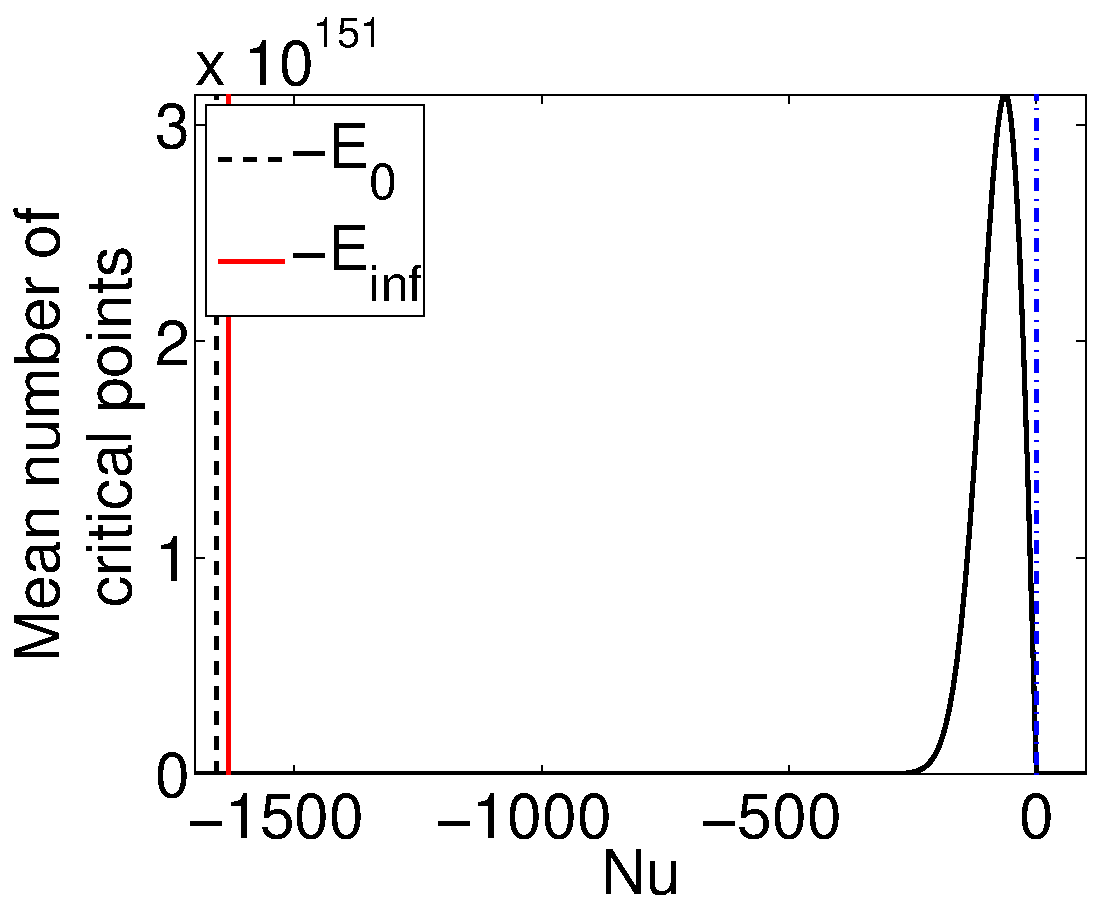
\includegraphics[width = 1.65in]{Distr_cp.pdf}
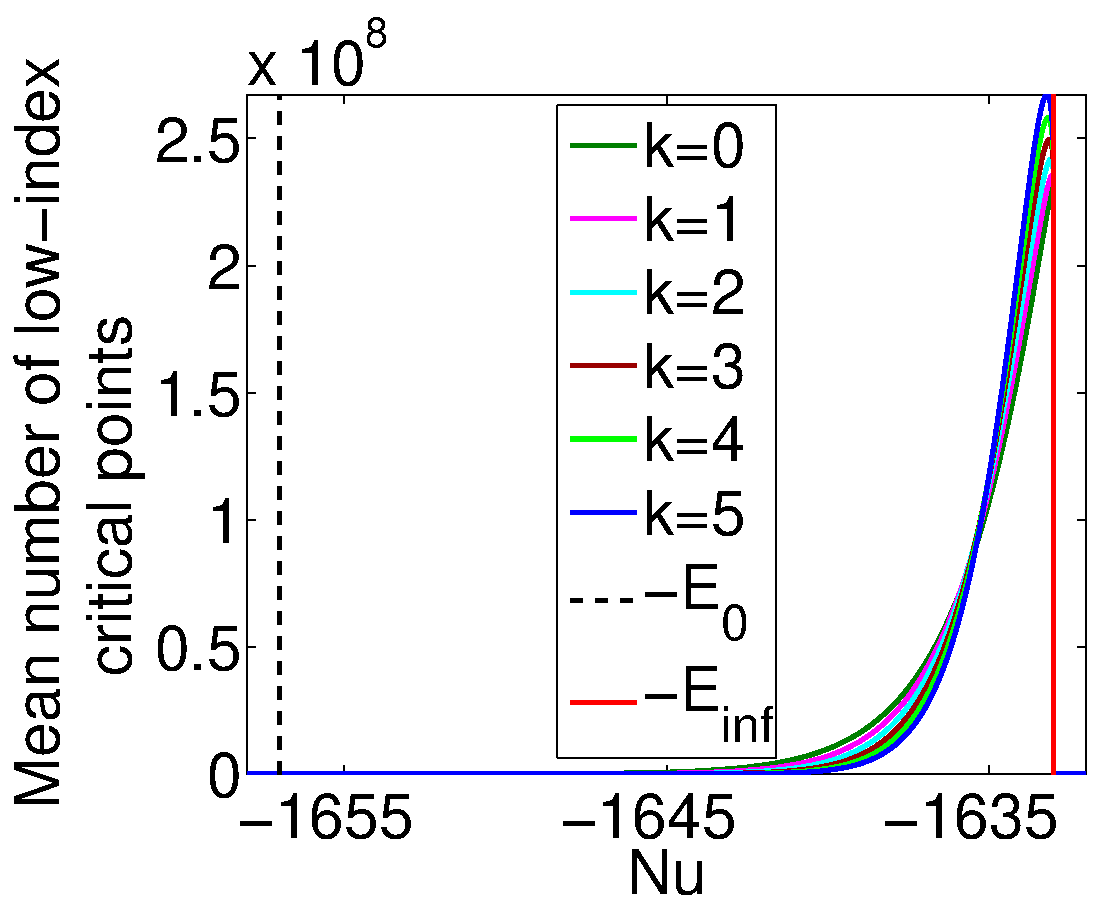
\includegraphics[width = 1.65in]{Distr_lm_sp_li.pdf} 
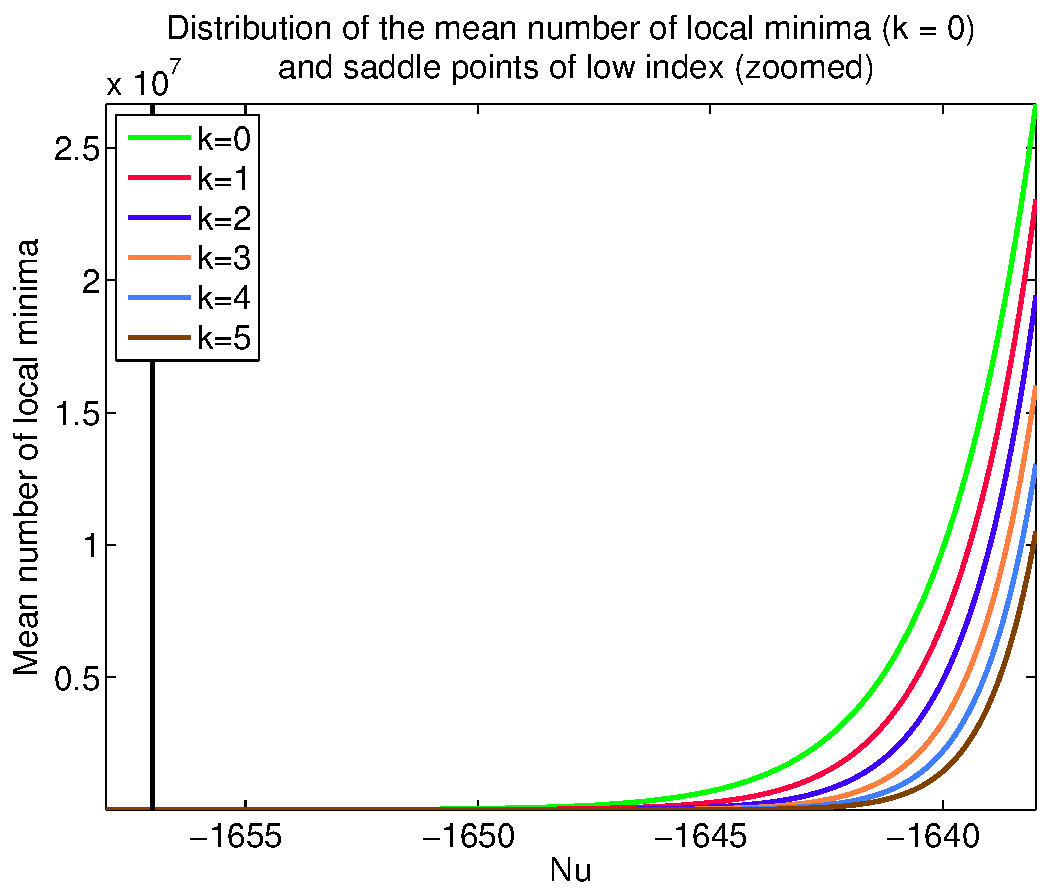
\includegraphics[width = 1.65in]{Distr_lm_sp_li_zoomed_left.pdf} 
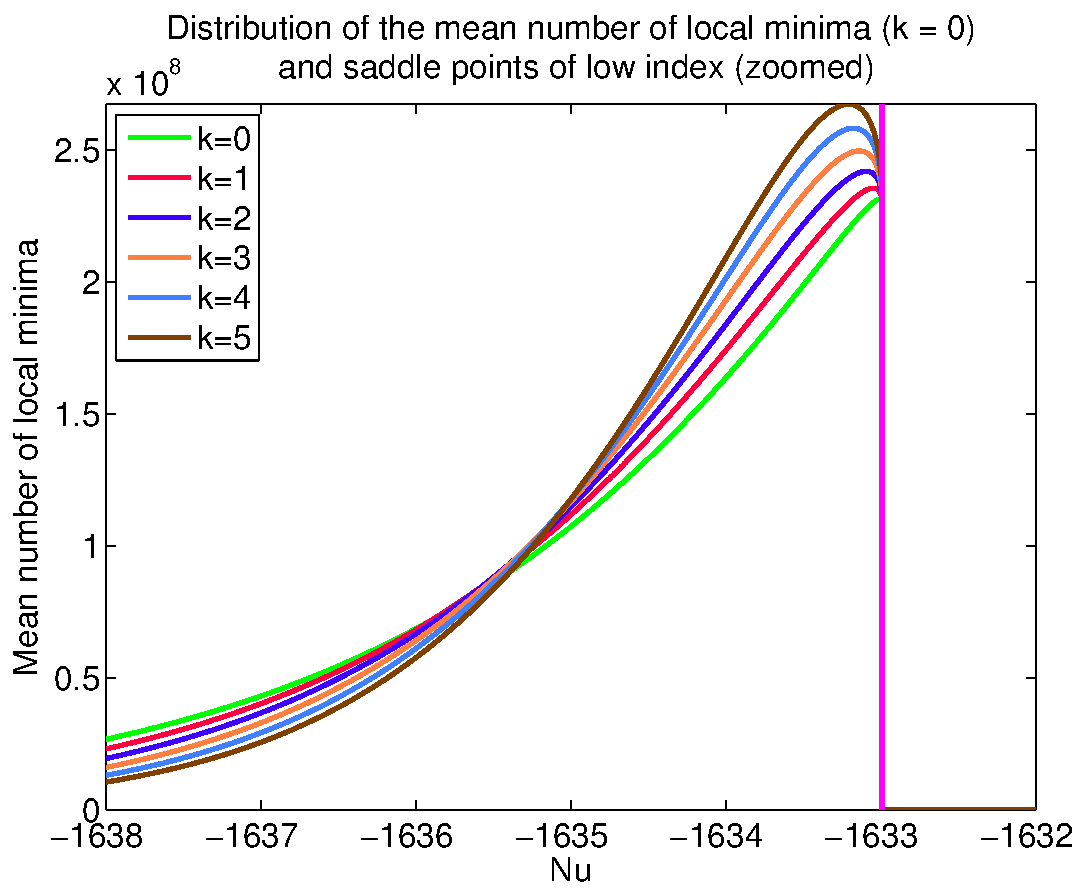
\includegraphics[width = 1.65in]{Distr_lm_sp_li_zoomed_right.pdf} 
\vspace{-0.3in}
\caption{Distribution of the mean number of critical points, local minima and low-index saddle points (oryginal and zoomed). Parameters $H$ and $\Lambda$ were set to $H = 3$ and $\Lambda = 1000$. Black line: $u = -E_0(H)$, red line: $u = -E_{\infty}(H)$. Figure must be read in color.}
\label{fig:Distr_cp_lm_sp}
\vspace{-0.1in}
\end{figure*}

\paragraph{Layered structure of low-index critical points}
From Theorem 2.15 in~\cite{AAC2010} it follows that for large-size networks finding a critical value with index larger or equal to $k$ (for any fixed integer $k$) below energy level $-\Lambda E_k(H)$ is improbable, where $-E_k(H) \in [-E_0(H),-E_{\infty}(H)]$. Furthermore, for any fixed $H \geq 3$, the sequence $\{E_k(H)\}_{k\in\mathbb{N}}$ is strictly decreasing and converges to $E_{\infty}$ as $k \rightarrow \infty$~\cite{AAC2010}. 

These results unravel a layered structure for the lowest critical values of the loss function of a large-size network, where with overwhelming probability the critical values above the global minimizer (ground state) of the loss function are local minima exclusively. Above the band ($\left(-\Lambda E_0(H),-\Lambda E_1(H)\right)$) containing only local minima (critical points of index $0$), there is another one, ($\left(-\Lambda E_1(H),-\Lambda E_2(H)\right)$), where one can only find local minima and saddle points of index $1$, and above this band there exists another one, ($\left(-\Lambda E_2(H),-\Lambda E_3(H)\right)$), where one can only find local minima and saddle points of index $1$ and $2$, etc. 

The band $(-E_0(H),-E_{\infty})$ is in practice very narrow, i.e. it is order of magnitudes narrower than band $(-E_{\infty},0)$ (an example is shown in Figure~\ref{fig:Distr_cp_lm_sp} and~\ref{fig:Thetas}). 

\paragraph{Hardness of recovering the global minimum}
Note that based on what was already shown recovering the global minimizer when starting from any (local) minima from one of the energy bands above, e.g. $\left(-\Lambda E_i(H),-\Lambda E_{i+1}(H)\right)$, diverges with $\Lambda$ since it is bounded below by $\Lambda (E_0(H) - E_i(H))$. \textcolor{red}{More should be written.}

\paragraph{Logarithmic asymptotics of the mean number of critical points}
We will now define two non-decreasing, continuous functions on $\mathbb{R}$, $\Theta_H$ and $\Theta_{k,H}$ as follows
\[\Theta_H(u) = \left \{
  \begin{tabular}{c}
  $\!\!\!\!\frac{1}{2}\log(H\!-\!1) \!-\! \frac{H-2}{4(H-1)} \!-\! I(u)$ $\:\:\:$if$\:\:$$u \!\leq\! -E_{\infty}$\\
  $\!\!\!\!\!\frac{1}{2}\log(H\!-\!1) \!-\! \frac{H-2}{4(H-1)}$ $\:\:\:\:\:\:$if$\:\:$$-E_{\infty} \!\leq\! u \leq 0$\\
  $\!\!\!\!\!\!\!\!\!\!\!\!\!\!\!\frac{1}{2}\log(H-1)$ $\:\:\:\:\:\:\:\:\:\:\:\:\:\:\:\:\:\:\:\:\:\:\:\:\:\:\:\:\:\:\:$if$\:\:$$0 \!\leq\! u$
  \end{tabular}
\right.,
\]
and for any integer $k \geq 0$:
\[\Theta_{k,H}(u) \!=\! \left \{
  \begin{tabular}{c}
  $\!\!\!\!\!\frac{1}{2}\!\log(\!H\!-\!1\!) \!-\! \frac{H\!-\!2}{4(\!H-1\!)} \!-\! (k\!+\!1)I(u)$ if$\:$$u \!\!\leq\!\! -E_{\infty}$\\
  $\!\!\!\!\frac{1}{2}\log(\!H\!-\!1\!) \!-\! \frac{H\!-\!2}{4(\!H-1\!)}$ $\:\:\:\:\:\:\:\:\:\:\:\:\:\:\:\:\:\:\:\:\:\:\:\:$if$\:$$u \!\!\geq\!\! -E_{\infty}$
  \end{tabular}
\right.
\]
where 
\[I(u) = -\frac{u}{E_{\infty}^2}\sqrt{u^2 \!-\! E_{\infty}^2} - \log(-u + \sqrt{u^2 \!-\! E_{\infty}^2}) + \log E_{\infty}.
\]
Note that the maximal values of $\Theta_H(u)$ and $\Theta_{k,H}(u)$ are respectively $\frac{1}{2}\log(H-1)$ and $\frac{1}{2}\log(H-1) - \frac{H-2}{H}$. Figure~\ref{fig:Thetas} captures exemplary plots of the functions $\Theta_H(u)$ and $\Theta_{k,H}(u)$. Also note that the following corollary holds.

\begin{figure}[h]
  \center
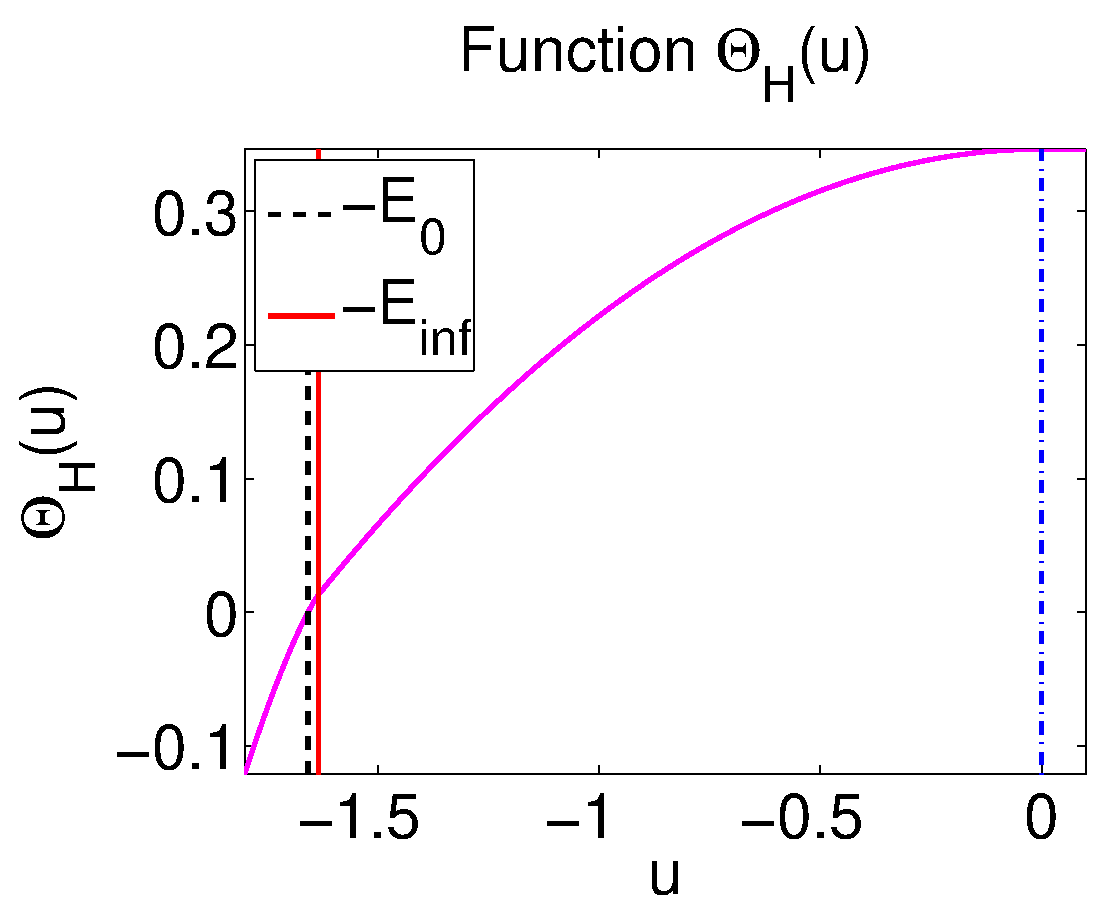
\includegraphics[width = 1.6in]{Theta_cp.pdf}
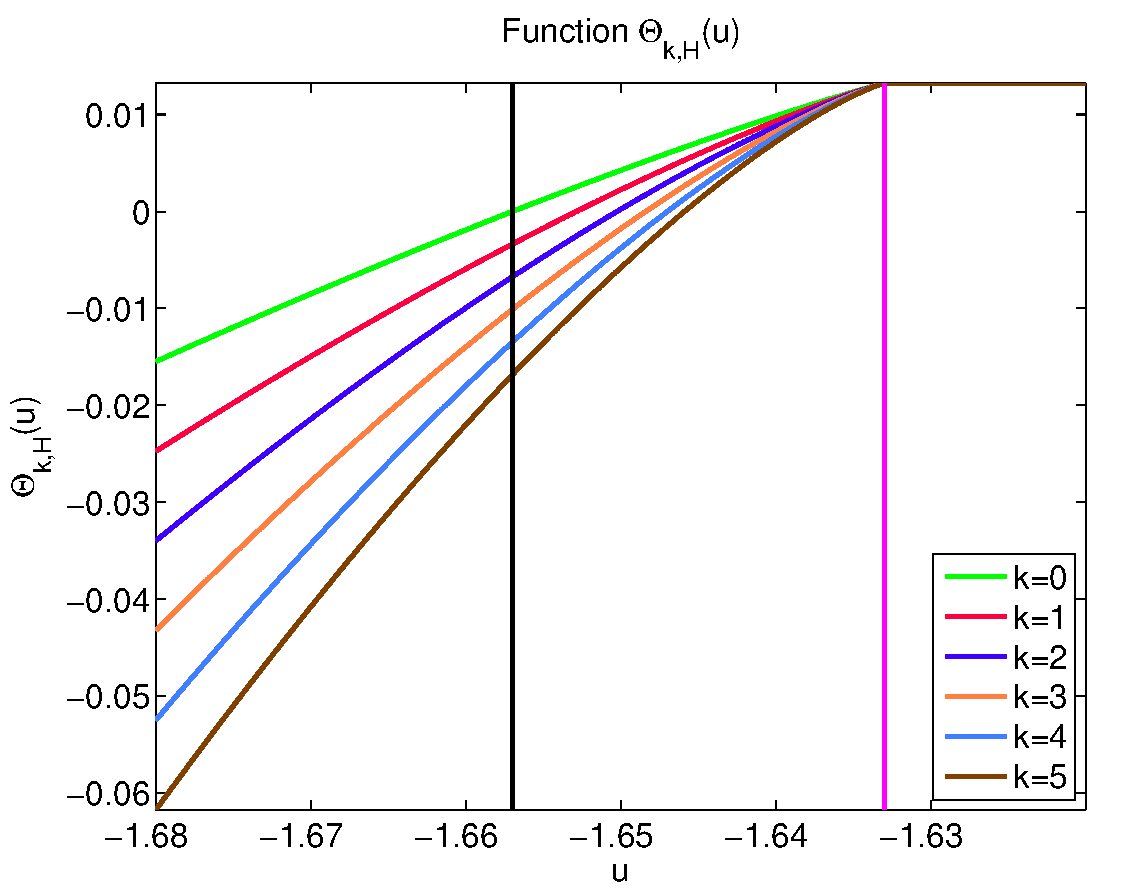
\includegraphics[width = 1.6in]{Theta_lm_sp.pdf}
\vspace{-0.3in}
\caption{Functions $\Theta_H(u)$ and $\Theta_{k,H}(u)$ for $k = \{0,1,\dots,5\}$. Parameter $H$ was set to $H = 3$. Black line: $u = -E_0(H)$, red line: $u = -E_{\infty}(H)$. Notice how narrow band $(-E_0(H),-E_{\infty})$ is. Figure must be read in color.}
\label{fig:Thetas}
%\vspace{-0.05in}
\end{figure}

\begin{corollary}
For all $k > 0$ and $u < -E_{\infty}$, $\Theta_{k,H}(u) < \Theta_{0,H}(u)$.
\label{cor:Theta}
\end{corollary}

Next we will show the logarithmic asymptotics of the mean number of critical points (the asymptotics of the mean number of critical points can be found in the Supplementary material). 
\begin{theorem}[\cite{AAC2010}, Theorem 2.5 and 2.8]
For all $H \geq 2$
\[\lim_{\Lambda \rightarrow \infty}\frac{1}{\Lambda}\log\mathbb{E}[\mathcal{C}_{\Lambda}(u)] = \Theta_{H}(u).
\]
and for all $H \geq 2$ and $k \geq 0$ fixed
\[\lim_{\Lambda \rightarrow \infty}\frac{1}{\Lambda}\log\mathbb{E}[\mathcal{C}_{\Lambda,k}(u)] = \Theta_{k,H}(u).
\]
\label{thm:lmsp}
\end{theorem}
Note that from Theorem~\ref{thm:lmsp} and Corollary~\ref{cor:Theta} it follows that the number of critical points in the band $\left(-\Lambda E_0(H),-\Lambda E_{\infty}(H)\right)$ increases exponentially as $\Lambda$ grows and that local minima dominate over saddle points and this domination also grows exponentially as $\Lambda$ grows. Thus for large-size networks (large $\Lambda$) the probability of recovering a saddle point in the band $\left(-\Lambda E_0(H),-\Lambda E_{\infty}(H)\right)$, rather than a local minima, goes to $0$.

Figure~\ref{fig:Distr_cp_lm_sp} captures exemplary plots of the distributions of the mean number of critical points, local minima and low-index saddle points. Clearly local minima and low-index saddle points are located in the band $\left(-\Lambda E_0(H),-\Lambda E_{\infty}(H)\right)$ whereas high-index saddle points can only be found above the energy barrier $-\Lambda E_{\infty}(H)$. Figure~\ref{fig:Distr_cp_lm_sp} also reveals the layered structure for the lowest critical values of the loss function. 

\section{Experiments}
\label{sec:Experiments}

\textcolor{red}{We need to prove that we get ot local minima not flat saddle points from Bengio paper.}

\section{Conclusion and Future Work}
\label{sec:ConandFutWork}

\bibliographystyle{apalike}
\bibliography{PAPER_AMMLY}

\clearpage

\toptitlebar 
{\Large \bf  \centering{Deep-optimization with large networks\\(Supplementary Material)} \par}
\bottomtitlebar

\section{Proof of Theorem~\ref{thm:arge}}
\begin{proof}
First we will prove the lower-bound on $N$. By the inequality between arithmetic and geometric mean the mass and the size of the network are connected as follows
\[N \geq \sqrt[H]{\Psi^2}\frac{H}{\sqrt[H]{n_0n_H}} = \sqrt[H]{\Psi^2}\frac{H}{\sqrt[H]{d}},
\]
and since $\sqrt[H]{\Psi}\frac{H}{\sqrt[H]{d}} = \sqrt[H]{\prod_{i = 1}^{H}n_i}H \geq 1$ then 
\[N \geq \sqrt[H]{\Psi^2}\frac{H}{\sqrt[H]{d}} \geq \sqrt[H]{\Psi}.
\]
Next we show the upper-bound on $N$. Let $n_{max} = \max_{i \in \{1,2,\dots,H\}}n_i$. Then
\[N \leq Hn_{max}^2 \leq H\Psi^2.
\]
\end{proof}

\section{Proof of Theorem~\ref{thm:redun}}
\begin{proof}
We will first proof the following more general lemma.
\begin{lemma}
Let $Y_1$ and $Y_2$ be the outputs of two arbitrary binary classifiers. Assume that the first classifiers predicts $1$ with probability $p$ where, without loss of generality, we assume $p \leq 0.5$ and $-1$ otherwise. Furthemore, let the prediction accuracy of the second classifier differ from the prediction accuracy of the first classifier by no more than $\epsilon \in [0,p]$. Then the following holds
\[corr(sign(Y_1),sign(Y_2))
\]
\[\geq \frac{1 - 2\epsilon - (1 - 2p)^2 - 2(1 - 2p)\epsilon}{4\sqrt{p(1 - p)(p + \epsilon)(1 - p + \epsilon)}}.
\]
\end{lemma}
\begin{proof}
Consider two random variables $Z_1 = sign(Y_1)$ and $Z_2 = sign(Y_2)$. Let $\mathcal{X}^{+}$ denote the set of data points for which the first classifier predicts $+1$ and let $\mathcal{X}^{-}$ denote the set of data points for which the first classifier predicts $-1$ ($\mathcal{X}^{+} \cup \mathcal{X}^{-} = \mathcal{X}$, where $\mathcal{X}$ is the entire dataset). Also let $p = \frac{|\mathcal{X}^{+}|}{|\mathcal{X}|}$. Furthermore, let $\mathcal{X}_{\epsilon}^{-}$ denote the dataset for which $Z_1 = +1$ and $Z_2 = -1$ and $\mathcal{X}_{\epsilon}^{+}$ denote the dataset for which $Z_1 = -1$ and $Z_2 = +1$, where $\frac{|\mathcal{X}_{\epsilon}^{+}| + |\mathcal{X}_{\epsilon}^{-}|}{\mathcal{X}} = \epsilon$. Also let $\epsilon^{+} = \frac{|\mathcal{X}_{\epsilon}^{+}|}{\mathcal{X}}$ and $\epsilon^{-} = \frac{|\mathcal{X}_{\epsilon}^{-}|}{\mathcal{X}}$. Therefore
\[Z_1 \!=\! \left \{
  \begin{tabular}{c}
  $1$ \:\:if $x \in \mathcal{X}^{+}$\\
  \!\!\!\!$-1$ \:\:if $x \in \mathcal{X}^{-}$
  \end{tabular}
\right.
\]
and
\[Z_2 \!=\! \left \{
  \begin{tabular}{c}
  $1$ \:\:if $x \in \mathcal{X}^{+} \cup \mathcal{X}_{\epsilon}^{+}  \setminus \mathcal{X}_{\epsilon}^{-}$\\
  \!\!\!$-1$ \:\:if $x \in \mathcal{X}^{-} \cup \mathcal{X}_{\epsilon}^{-} \setminus \mathcal{X}_{\epsilon}^{+}$.
  \end{tabular}
\right.
\]
One can compute that $\mathbb{E}[Z_1] = 2p-1$, $\mathbb{E}[Z_2] = 2(p + \epsilon^{+} - \epsilon^{-}) - 1$, $\mathbb{E}[Z_1Z_2] = 1 - 2\epsilon$, $std(Z_s) = 2\sqrt{p(1-p)}$, and finally $std(Z_\Lambda) = 2\sqrt{(p + \epsilon^{+} - \epsilon^{-})(1 - p - \epsilon^{+} + \epsilon^{-})}$.
Thus we obtain
\begin{eqnarray}
&&\!\!\!\!\!\!\!\!\!\!\!\!\!\!\!corr(sign(Y_1),sign(Y_2)) = corr(Z_1,Z_2) \nonumber\\
&\!\!\!\!\!\!\!\!\!\!\!\!\!\!\!=& \!\!\!\!\!\!\!\!\!\!\frac{\mathbb{E}[Z_1Z_2] - \mathbb{E}[Z_1]\mathbb{E}[Z_2]}{std(Z_1)std(Z_2)} \nonumber\\
&\!\!\!\!\!\!\!\!\!\!\!\!\!\!\!=& \!\!\!\!\!\!\!\!\!\!\frac{1 - 2\epsilon - (1 - 2p)^2 + 2(1 - 2p)(\epsilon^{+} - \epsilon^{-})}{4\sqrt{p(1 - p)(p + \epsilon^{+} - \epsilon^{-})(1 - p - \epsilon^{+} + \epsilon^{-})}} \nonumber\\
&\!\!\!\!\!\!\!\!\!\!\!\!\!\!\!\geq& \!\!\!\!\!\!\!\!\!\!\frac{1 - 2\epsilon - (1 - 2p)^2 - 2(1 - 2p)\epsilon}{4\sqrt{p(1 - p)(p + \epsilon)(1 - p + \epsilon)}}
\label{eq:tmp}
\end{eqnarray}
\end{proof}
Note that when the first classifier is network $\mathcal{N}$ considered in this paper and $\mathcal{M}$ is its $(s,\epsilon)$-reduction image $\mathbb{E}[Y_1] = 0$ and $\mathbb{E}[Y_2] = 0$ (that follows from the fact that $X$'s in Equation~\ref{eq:befapprox} have zero-mean). That implies $p=0.5$ which, when substituted to Equation~\ref{eq:tmp} gives the theorem statement.
\end{proof}

\section{Proof of Theorem~\ref{thm:unif}}
\begin{proof}
Note that $\mathbb{E}[\hat{Y}_s] = 0$ and $\mathbb{E}[Y_s] = 0$. Furthermore
\[\mathbb{E}[\hat{Y}_sY_{\Lambda}] = q^2\rho^2\!\!\!\sum_{i_1,i_2,\dots,i_H=1}^{\Lambda}\!\!\!\min\left(\frac{\Psi}{\Lambda^H},t_{i_1,i_2,\dots,i_H}\right)\prod_{k = 1}^{H}w_{i_k}^2
\]
and
\[std(\hat{Y}_s) = q\rho\sqrt{\sum_{i_1,i_2,\dots,i_H=1}^{\Lambda}\frac{\Psi}{\Lambda^H}\prod_{k = 1}^{H}w_{i_k}^2}
\]
\[std(Y_s) = q\rho\sqrt{\sum_{i_1,i_2,\dots,i_H=1}^{\Lambda}t_{i_1,i_2,\dots,i_H}\prod_{k = 1}^{H}w_{i_k}^2}.
\]
Therefore
\begin{eqnarray*}
&&\!\!\!\!\!\!\!\!\!corr(\hat{Y}_s,Y_s)\\ 
&\!\!\!\!\!\!\!\!\!=&\!\!\!\!\!\!\! \frac{\displaystyle\sum_{i_1,\dots,i_H=1}^{\Lambda}\min\left(\frac{\Psi}{\Lambda^H},t_{i_1,\dots,i_H}\right)\prod_{k = 1}^{H}w_{i_k}^2}{\sqrt{\!\!\!\left(\displaystyle\sum_{i_1,\dots,i_H=1}^{\Lambda}\frac{\Psi}{\Lambda^H}\prod_{k = 1}^{H}w_{i_k}^2\right)\!\!\!\!\left(\displaystyle\sum_{i_1,\dots,i_H=1}^{\Lambda}\!\!\!\!\!t_{i_1,\dots,i_H}\prod_{k = 1}^{H}w_{i_k}^2\right)}}\\
&\!\!\!\!\!\!\!\!\geq& \frac{1}{c^2}, 
\end{eqnarray*}
where the last inequality is the direct consequence of the uniformity assumption of Equation~\ref{eq:uniform}.
\end{proof}

\section{Loss function as a $H$ - spin spherical spin-glass model}

We consider two loss functions, (random) absolute loss $\mathcal{L}^a_{\Lambda,H}(w)$ and (random) hinge loss $\mathcal{L}^h_{\Lambda,H}(w)$ defined as
\[\mathcal{L}^a_{\Lambda,H}({\bm w}) = |Y_t - \hat{Y}_s|
\]
and
\[\mathcal{L}^h_{\Lambda,H}({\bm w}) = \max(0,1-Y_t\hat{Y}_s).
\]
where $Y_t$ is a random variable corresponding to the true data labeling that takes values $-S$ or $S$ in case of the absolute loss and $-1$ or $1$ in case of the hinge loss, where $S = \sup_{\bf{w}}{\hat{Y}_s}$. Note that in case of the hinge loss $\max$ operator can be modelled as Bernoulli random variable, that we will refer to as $M$, with success ($M = 1$) probability $\rho^{'} = \frac{\mathcal{C}^{'}}{\rho\sqrt{\mathcal{C}^H}}$ for some non-negative constant $\mathcal{C}^{'}$. We assume $M$ is independent of $\hat{Y}_s$. Therefore we obtain that
\[\mathcal{L}^a_{\Lambda,H}({\bm w}) = \left \{
  \begin{tabular}{c}
  $\!\!\!\!\!\!S - \hat{Y}_s$ $\:\:\:\:$if$\:\:\:\:$ $Y_t = S$ \\
  $\!S + \hat{Y}_s$ $\:\:\:\:$if$\:\:\:\:$ $Y_t = -S$ \\
  \end{tabular}
\right.
\]
and
\begin{eqnarray*}
\mathcal{L}^h_{\Lambda,H}({\bm w}) &=& \mathbb{E}_{M,A}[M(
1-Y_t\hat{Y}_s)]\\&=& \left \{
  \begin{tabular}{c}
  $\!\!\!\!\!\!\mathbb{E}_{M}[M(1 - \hat{Y}_s)]$ $\:\:\:\:$if$\:\:\:\:$ $Y_t = 1$ \\
  $\!\mathbb{E}_{M}[M(1 + \hat{Y}_s)]$ $\:\:\:\:$if$\:\:\:\:$ $Y_t = -1$ \\
  \end{tabular}
\right.
\end{eqnarray*}
Note that both cases can be generalized as
\[\mathcal{L}_{\Lambda,H}({\bm w}) = \left \{
  \begin{tabular}{c}
  $\!\mathbb{E}_{M}[M(S - \hat{Y}_s)]$ $\:\:\:\:$if$\:\:\:\:$ $Y_t  > 0$ \\
  $\!\mathbb{E}_{M}[M(S + \hat{Y}_s)]$ $\:\:\:\:$if$\:\:\:\:$ $Y_t < 0$ \\
  \end{tabular}
\right.,
\]
where in case of the absolute loss $\rho^{'} = 1$ and in case of the hinge loss $S = 1$. Furthermore, using the fact that $X$'s are Gaussian random variables one we can further generalize both cases as
\[\mathcal{L}_{\Lambda,H}({\bm w}) = S\rho^{'} \!+\! q\sum_{i_1,i_2,\dots,i_H=1}^{\Lambda}\!\!\!\!\!\!\!X_{i_1,i_2,\dots,i_H}\rho\rho^{'}\prod_{k = 1}^{H}w_{i_k}.
\]
Let $\tilde{w}_i = \sqrt[H]{\frac{\rho\rho^{'}}{\mathcal{C}^{'}}}w_i$ for all $i = \{1,2,\dots,k\}$. Note that $\tilde{w}_i = \frac{1}{\sqrt{C}}w_i$. Thus
\begin{equation}
\mathcal{L}_{\Lambda,H}({\bm w}) = S\rho^{'} + q\mathcal{C}^{'}\sum_{i_1,\dots,i_H=1}^{\Lambda}X_{i_1,\dots,i_H}\prod_{k = 1}^{H}\tilde{w}_{i_k}.
\label{eq:befloss}
\end{equation}
Note that the spherical assumption in Equation~\ref{eq:befspherical} directly implies that
\begin{equation*}
\frac{1}{\Lambda}\sum_{i=1}^{\Lambda}\tilde{w}_i^2 = 1
\end{equation*}
To simplify the notation in Equation~\ref{eq:befloss} we drop the letter accents and simply denote $\hat{w}$ as $w$. We skip constant $S\rho^{'}$ and $\mathcal{C}^{'}$ as it does not matter when minimizing the loss function. After substituting $q = \frac{1}{\Psi^{(H-1)/2H}}$ we obtain
\begin{equation*}
\mathcal{L}_{\!\Lambda,H}({\bm w}) \!=\! \frac{1}{\Lambda^{\!(H\!-\!1)/2}}\!\!\!\!\!\!\!\sum_{i_1,i_2,\dots,i_H=1}^{\Lambda}\!\!\!\!\!\!\!\!\!\!\!X_{i_1,i_2,\dots,i_H}\!w_{i_1}\!w_{i_2}\!\!\dots\!w_{i_H}.
\end{equation*}

\section{Asymptotics of the mean number of critical points and local minima}

Below, we provide the asymptotics of the mean number of critical points (Theorem~\ref{thm:cpprecise}) and the mean number of local minima (Theorem~\ref{thm:lmspprecise}), which extend Theorem~\ref{thm:lmsp}. Those results are the consequences of Theorem 2.17. and Corollary 2.18.~\cite{AAC2010} and the boundeness of $c$ and $H$.
\begin{theorem}
For $H \geq 3$, the following holds as $\Lambda \rightarrow \infty$:
\begin{itemize}
\item For $u < -E_{\infty}$\\
\begin{eqnarray*}
\mathbb{E}[\mathcal{C}_{\Lambda}(u)] \!\!\!&=&\!\!\! \frac{h(v)}{\sqrt{2H\pi}}\frac{\exp(I_1(v) - \frac{v}{2}I_1^{'}(v))}{-\Phi^{'}(v) + I_1^{'}(v)}\Lambda^{-\frac{1}{2}}\\
&\cdot& \exp\left(\Lambda\Theta_H(u)\right)(1 + o(1)),
\end{eqnarray*}
where $v = -u\sqrt{\frac{H}{2(H-1)}}$, $\Phi(v) = -\frac{H-2}{2H}v^2$,\\
$h(v) = \left|\frac{v-\sqrt{2}}{v + \sqrt{2}}\right|^{\frac{1}{4}} + \left|\frac{v+\sqrt{2}}{v - \sqrt{2}}\right|^{\frac{1}{4}}$\\
and $I_1(v) = \int_{\sqrt{2}}^{v}\sqrt{|x^2 - 2|}dx$.
\item For $u = -E_{\infty}$\\
\begin{eqnarray*}
\mathbb{E}[\mathcal{C}_{\Lambda}(u)] = \frac{2A(0)\sqrt{2H}}{3(H-2)}\Lambda^{-\frac{1}{3}}\\
\cdot\exp\left(\Lambda\Theta_H(u)\right)(1 + o(1)),
\end{eqnarray*}
where $A$ is the Airy function of first kind.
\item For $u \in (-E_{\infty},0)$\\
\begin{eqnarray*}
\mathbb{E}[\mathcal{C}_{\Lambda}(u)] = \frac{2\sqrt{2H(E_{\infty}^2-u^2)}}{(2-H)\pi u}\\
\cdot\exp\left(\Lambda \Theta_H(u)\right)(1 + o(1)),
\end{eqnarray*}
\item For $u > 0$\\
\begin{eqnarray*}
\mathbb{E}[\mathcal{C}_{\Lambda}(u)] = \frac{4\sqrt{2}}{\sqrt{\pi(H-2)}}\Lambda^{\frac{1}{2}}\\
\cdot\exp\left(\Lambda\Theta_H(0)\right)(1 + o(1)),
\end{eqnarray*}
\end{itemize}
\label{thm:cpprecise}
\end{theorem}
\begin{theorem}
For $H \geq 3$ and $u < -E_{\infty}$, the following holds as $\Lambda \rightarrow \infty$:
\begin{eqnarray*}
\mathbb{E}[\mathcal{C}_{\Lambda,0}(u)] \!\!\!&=&\!\!\! \frac{h(v)}{\sqrt{2H\pi}}\frac{\exp(I_1(v) - \frac{v}{2}I_1^{'}(v))}{-\Phi^{'}(v) + I_1^{'}(v)}\Lambda^{-\frac{1}{2}}\\
&\cdot& \exp\left(\Lambda\Theta_H(u)\right)(1 + o(1)),
\end{eqnarray*}
where $v$, $\Phi$, $h$ and $I_1$ were defined in Theorem~\ref{thm:cpprecise}.
\label{thm:lmspprecise}
\end{theorem}

\end{document}
